\documentclass[english,serif,mathserif,xcolor=pdftex,dvipsnames,table]{beamer}

\usepackage[T1]{fontenc}
\usepackage[utf8x]{inputenc}

\usetheme[informal]{s3it}
\usepackage{s3it}

\title[Getting started]{%
  A Short and Incomplete Introduction to Julia
}
\subtitle{\bfseries Part 0: Introduction}
\author[R.~Murri]{%
  \textbf{Riccardo Murri} \texttt{<riccardo.murri@uzh.ch>}
  \\
  S3IT: Services and Support for Science IT,
  \\
  University of Zurich
}
\date{September 12, 2019}


\begin{document}

% title frame
\maketitle

\begin{frame}
  \begin{center}
    {\Huge Welcome!}
  \end{center}
\end{frame}


\begin{frame}
  \frametitle{Prerequisites}
  This course assumes a basic experience with computer programming.

  \+
  Any language should do, as long as you are already familiar with
  the concepts of variables and functions.
\end{frame}


\begin{frame}
  \begin{center}
    {\Huge What about you?}
    \\ \+ \+
    \small
    Name \textbf{/}
    Affiliation \textbf{/}
    Interest in Julia?~\textbf{/}
    \\
    Other known programming languages?
  \end{center}
\end{frame}


\begin{frame}
  \frametitle{Course outline}
  \begin{enumerate}
  \item Julia basics
  \item Array manipulation and plotting
  \item How to query tabular data
  %\item Distributed computing
  \end{enumerate}
\end{frame}


\begin{frame}
  \frametitle{Next steps}

  The course will be structured as a mixture of slides and hands-on
  sessions for practicing Julia programming.

  \+
  So, the very first step is making sure you can access the Jupyter
  server for running the exercise notebooks.
\end{frame}


\part{How to run Julia code}

\begin{frame}
  \frametitle{The Jupyter notebook, I}

  \begin{columns}[t]
    \begin{column}{0.5\textwidth}
      \begin{center}
        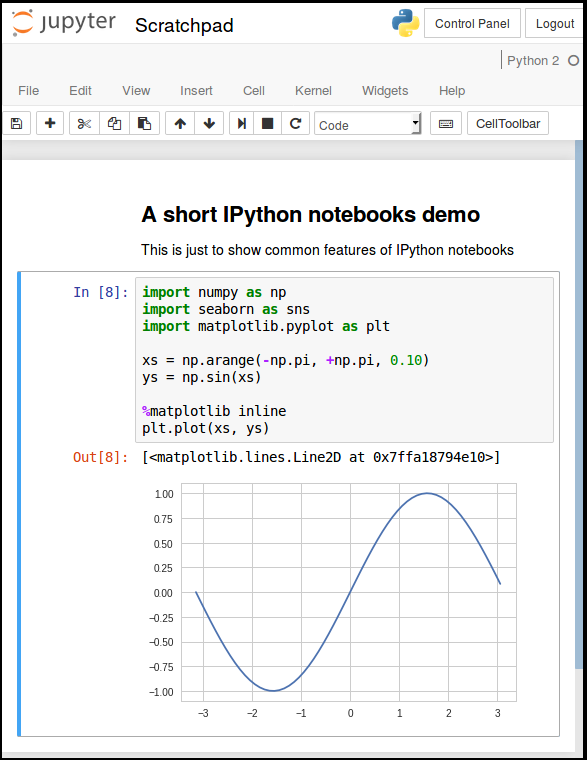
\includegraphics[width=1.00\linewidth]{fig/nb.png}
      \end{center}
    \end{column}
    \begin{column}{0.5\textwidth}
      \small

      An appealing way of interacting with Julia
      is through \emph{Jupyter notebooks}.

      \+
      Notebooks are made of ``cells'', which come in two flavors:
      \begin{itemize}
      \item documentation cells, containing text formatted according to the
        \href{http://commonmark.org/help/}{Markdown} conventions;
      \item code cells, containing arbitrary Julia code
      \end{itemize}
    \end{column}
  \end{columns}
\end{frame}


\begin{frame}
  \frametitle{The Jupyter notebook, II}

  To run Julia code in the notebook:
  \begin{itemize}
  \item Type your code in a cell besides the {\ttfamily\bfseries\color{blue}
      In~[~]:} (multiple lines are allowed)
  \item Press \textbf{Ctrl+Enter} to evaluate the cell (prompt changes to
    {\ttfamily\bfseries\color{blue} In~[*]:}) --- or press \textbf{Alt+Enter} to
    evaluate the code \emph{and} open a new code cell.
  \item When the Julia kernel has done computing, the result appears \emph{under} the
    code cell marked with a {\ttfamily\bfseries\color{red} Out~[~]:} label.
  \end{itemize}

\end{frame}


\begin{frame}[fragile]
  \frametitle{The Julia REPL, I}
  Julia features an interactive
  \href{http://en.wikipedia.org/wiki/REPL}{``shell''} for evaluating
  expressions and statements immediately.

  \+
  Julia interaction is started by invoking the command
  \texttt{julia} in a terminal window.

  \+
\begin{semiverbatim}\tiny
\$ \textbf{julia}
               _
   _       _ _(_)_     |  Documentation: https://docs.julialang.org
  (_)     | (_) (_)    |
   _ _   _| |_  __ _   |  Type "?" for help, "]?" for Pkg help.
  | | | | | | |/ _` |  |
  | | |_| | | | (_| |  |  Version 1.2.0 (2019-08-20)
 _/ |{\textbackslash}__'_|_|_|{\textbackslash}__'_|  |  Official https://julialang.org/ release
|__/                   |

\textbf{julia>}{\color{blue}\normalfont\em \(\leftarrow\) this is where you enter commands}
\end{semiverbatim}
\end{frame}


\begin{frame}[fragile,fragile]
  \frametitle{The Julia REPL, II}
  \smaller

  Expressions can be entered at the Julia REPL prompt; they are evaluated and the
  result is printed:
\begin{semiverbatim}
\In 2+2
\Out 4
\end{semiverbatim}

  \+
  (The acronym REPL indeed means ``Read-Eval-Print-Loop''.)

  \+ Throughout these slides, all code marked with either `{\color{blue}
    In~[*]}' or `\texttt{julia>}' can also be entered and evaluated in the Julia
  notebook cells.
\end{frame}


\begin{frame}[fragile]
  \frametitle{Getting help from Julia}
  Typing \texttt{?} followed by a word \\ searches the built-in help for
  that topic.
\begin{semiverbatim}\smaller
\In {\bfseries ?julia}
\Out
search:

  Welcome to Julia 1.2.0. The full manual is available at

  https://docs.julialang.org/

  {\itshape [...]}
\end{semiverbatim}

  Works both in the REPL and in the Notebook.

  \+ Use it to find help about any topic in Julia, especially built-in
  functions and types (e.g., try `\texttt{?print}').
\end{frame}

\end{document}

%%% Local Variables:
%%% mode: latex
%%% TeX-master: t
%%% End:
